%%
%% /docs/report/content/chapters/results.tex
%%
%% Created by Paul Warkentin <paul@warkentin.email> on 21/07/2018.
%% Updated by Paul Warkentin <paul@warkentin.email> on 26/07/2018.
%%

\section{Results}
\label{section:results}

In this section, the results of the training from the projects' implementation is discussed. The VGG 16 model was initialized with the pre-trained weights on the ILSVRC-2012-CLS\footnote{\url{http://www.image-net.org/challenges/LSVRC/2012/}} image classification dataset. The network was trained for research by TensorFlow-Slim \cite{slimmodels}.

\subsection{Training}

The SSD 300 network was trained for a total of 100k steps with batch size 32. One step is defined as one forward pass and one backward pass of the network. The loss was minimized using the Momentum optimizer with momentum value 0.9. For the learning rate decay, we used the following rule: the first 70k steps were trained with learning rate 1e-3, the next 15k steps with 1e-4 and the last 15k steps with 1e-5. This training process took about 24 hours. \\

The SSD 512 network was trained with batch size 16, the same optimizer settings and with learning rate 1e-3 for 100k steps, 1e-4 for 20k steps and 1e-5 for another 20k steps.

\bgroup
\vspace{\abovedisplayskip}
\begin{minipage}{0.5\textwidth}
  \begin{tikzpicture}[scale=0.75]
    \begin{axis}[
        xlabel = Step,
        ylabel = Loss
      ]
      \addplot[color=orange] table[col sep=comma,x=step,y=loss] {train_loss.dat};
      \addplot[color=blue] table[col sep=comma,x=step,y=loss] {eval_loss.dat};
    \end{axis}
  \end{tikzpicture}
\end{minipage}
\begin{minipage}{0.5\textwidth}
  \begin{tikzpicture}[scale=0.75]
    \begin{axis}[
        xlabel = Step,
        ylabel = mAP
      ]
      \addplot[color=orange] table[col sep=comma,x=step,y=map] {train_map.dat};
      \addplot[color=blue] table[col sep=comma,x=step,y=map] {eval_map.dat};
    \end{axis}
  \end{tikzpicture}
\end{minipage}
\captionof{figure}{SSD 300: Train (orange) and evaluation (blue) loss and mAP. The network starts to overfit although the dataset was heavily expanded using many data augmentation tricks.}
\vspace{\belowdisplayskip}
\egroup

Both networks were trained on the Pascal VOC 2007 + 2012 trainval dataset which is the union of the Pascal VOC 2007 \cite{voc2007} and Pascal VOC 2012 \cite{voc2012} trainval sets. The trained network was finally evaluated on the Pascal VOC 2007 test set.

\begin{center}
  \begin{tabular}{rl|c|r}
    & \textbf{Method} & \textbf{Dataset} & \textbf{mAP} \\ \cline{2-4}
    & Fast R-CNN & VOC 2007+2012 & 70.00\% \\
    & Faster R-CNN & VOC 2007+2012 & 76.80\% \\ \cline{2-4}
    & SSD 300 & VOC 2007+2012 & 74.30\% \\
    & SSD 512 & VOC 2007+2012 & 76.80\% \\ \cline{2-4}
    $\times$ & SSD 300 & VOC 2007+2012 & 49.09\% \\
    $\times$ & SSD 512 & VOC 2007+2012 & 54.37\%
  \end{tabular}
  \captionof{table}{mAP results compared to the original paper. The rows marked with $\times$ are the results from this project.}
\end{center}

When we look at the average precision values of each class, we can see that the network of this project can badly detect objects of the classes bottle, chair and potted plants. The following table compares the precision values of the implementation of this project to the values from the paper.

\begin{footnotesize}
  \begin{center}
    \setlength\tabcolsep{1pt}
    \begin{tabularx}{\textwidth}{rl|c|c|YYYYYYYYYY}
      & \textbf{Method} & \textbf{Data} & \textbf{mAP} & \textbf{aero} & \textbf{bike} & \textbf{bird} & \textbf{boat} & \textbf{bottle} & \textbf{bus} & \textbf{car} & \textbf{cat} & \textbf{chair} & \textbf{cow} \\ \cline{2-14}
      & SSD300 & 07+12 & 74.3 & 75.5 & 80.2 & 72.3 & 66.3 & 47.6 & 83.0 & \textbf{84.2} & \textbf{86.1} & 54.7 & 78.3 \\
      & SSD512 & 07+12 & 76.8 & 82.4 & 84.7 & 78.4 & 73.8 & 53.2 & \textbf{86.2} & \textbf{87.5} & \textbf{86.0} & 57.8 & 83.1 \\ \cline{2-14}
      $\times$ & SSD300 & 07+12 & 49.1 & 62.5 & 53.6 & 43.5 & 40.5 & 15.9 & 60.8 & 53.5 & \textbf{71.2} & 22.7 & 51.1 \\
      $\times$ & SSD512 & 07+12 & 54.4 & 63.0 & 64.2 & 53.6 & 41.0 & 27.8 & 63.8 & \textbf{71.2} & \textbf{80.7} & 33.6 & 48.2
    \end{tabularx}\vspace{10pt}
    \begin{tabularx}{\textwidth}{rl|c|c|YYYYYYYYYY}
      & \textbf{Method} & \textbf{Data} & \textbf{mAP} & \textbf{table} & \textbf{dog} & \textbf{horse} & \textbf{mbike} & \textbf{person} & \textbf{plant} & \textbf{sheep} & \textbf{sofa} & \textbf{train} & \textbf{tv} \\ \cline{2-14}
      & SSD300 & 07+12 & 74.3 & 73.9 & \textbf{84.5} & 85.3 & 82.6 & 76.2 & 48.6 & 73.9 & 76.0 & 83.4 & 74.0 \\
      & SSD512 & 07+12 & 76.8 & 70.2 & 84.9 & 85.2 & 83.9 & 79.7 & 50.3 & 77.9 & 73.9 & 82.5 & 75.3 \\ \cline{2-14}
      $\times$ & SSD300 & 07+12 & 49.1 & 41.8 & 60.9 & \textbf{62.6} & 60.3 & 51.0 & 22.9 & 43.3 & 41.8 & \textbf{70.2} & 51.8 \\
      $\times$ & SSD512 & 07+12 & 54.4 & 50.8 & 62.1 & 54.6 & 62.1 & 61.4 & 27.2 & 53.5 & 43.3 & \textbf{71.0} & 54.4
    \end{tabularx}
    \captionof{table}{Average precision results compared to the original paper. The 3 top values per method are highlighted. The rows marked with $\times$ are the results from this project.}
  \end{center}
\end{footnotesize}

Some reasons for the differences in the implementations may be the implementation of the pre-processing like data augmentation, computation of default anchor boxes and connected with that the matching strategy as well as the post-processing like selecting the final bounding boxes.

\subsection{Inference}

The original paper used a Titan X and cuDNN 4 with Intel Xeon E5-2667v3 @ 3.20GHz for inferece. The results of this project were tested using a GTX 1080 Ti and cuDNN 9.0 with Intel Core i7-6850K @ 3.60GHz. \\

In theory, both SSD networks have a higher mAP than other object detection models. With about 50 frames per second, SSD 300 delivers a good precision-speed ratio.

\begin{center}
  \begin{tabular}{rl|c|c|c|c|c}
    & \textbf{Method} & \textbf{mAP} & \textbf{FPS} & \textbf{BS} & \textbf{\# Boxes} & \textbf{Resolution} \\ \cline{2-7}
    & Faster R-CNN & 73.2\% & 7 & 1 & $\sim$ 6000 & $\sim$ 1000 $\times$ 600 \\ \cline{2-7}
    & Fast YOLO & 52.7\% & 155 & 1 & 98 & 448 $\times$ 448 \\
    & YOLO & 66.4\% & 21 & 1 & 98 & 448 $\times$ 448 \\ \cline{2-7}
    & SSD 300 & 74.3\% & 46 & 1 & 8732 & 300 $\times$ 300 \\
    & SSD 512 & 76.8\% & 19 & 1 & 24564 & 512 $\times$ 512 \\
    & SSD 300 & 74.3\% & 59 & 8 & 8732 & 300 $\times$ 300 \\
    & SSD 512 & 76.8\% & 22 & 8 & 24564 & 512 $\times$ 512 \\ \cline{2-7}
    $\times$ & SSD 300 & 49.09\% & 49 & 1 & 8732 & 300 $\times$ 300 \\
    $\times$ & SSD 512 & 54.37\% & 35 & 1 & 24564 & 512 $\times$ 512
  \end{tabular}
  \captionof{table}{Inference results compared to the original paper. The rows marked with $\times$ are the results from this project.}
\end{center}

\subsection{Sample images}

The following sample images were annotated using the SSD 300 network. The images are taken from the Pascal VOC 2007 test set which was also taken for the network evaluation. \\

Objects that stand alone seem to be detected better than objects that overlap with other objects. The combination of horses and people were detected very good in most of the times.

\bgroup
\setlength\tabcolsep{0pt}
\def\arraystretch{1}
\begin{center}
  \begin{tabular}[t]{cccc}
    \begin{tabular}{c}
      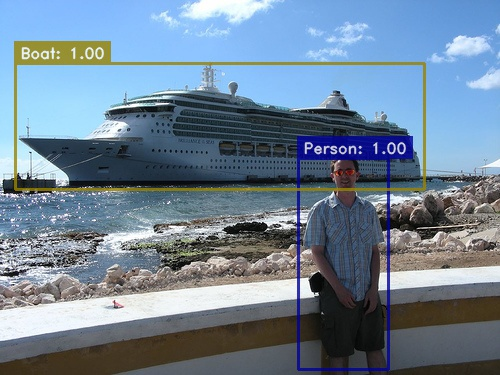
\includegraphics[width=0.2425\linewidth]{samples/good/000069.jpg} \\
      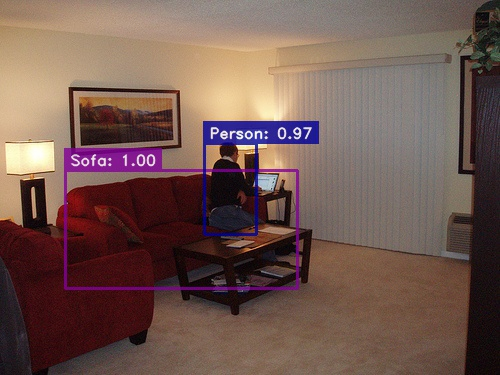
\includegraphics[width=0.2425\linewidth]{samples/good/000097.jpg} \\
      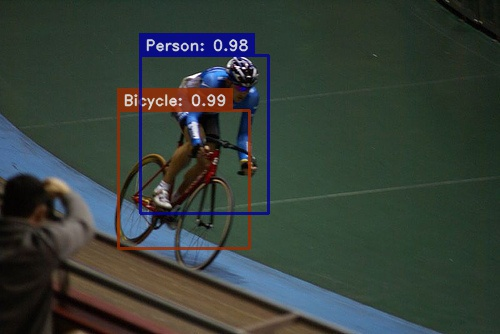
\includegraphics[width=0.2425\linewidth]{samples/good/000139.jpg} \\
      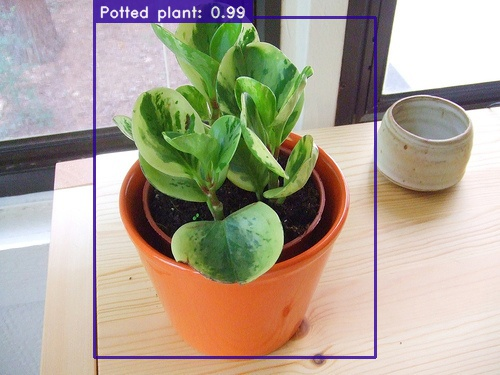
\includegraphics[width=0.2425\linewidth]{samples/good/000149.jpg}

    \end{tabular}\hspace{0.01\linewidth}
    &
    \begin{tabular}{c}
      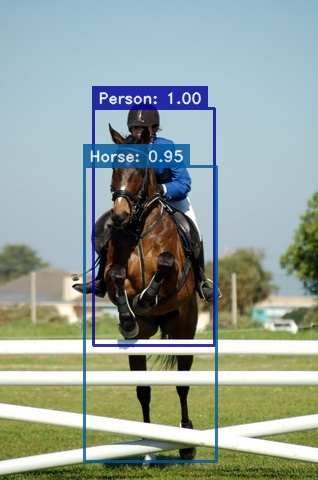
\includegraphics[width=0.2425\linewidth]{samples/good/000168.jpg} \\
      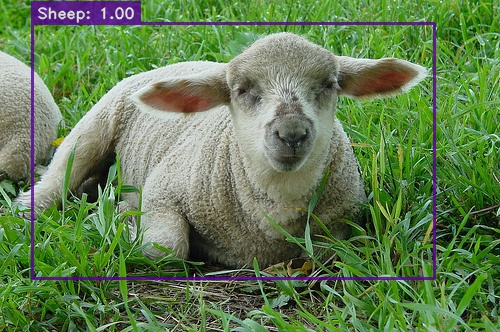
\includegraphics[width=0.2425\linewidth]{samples/good/000175.jpg} \\
      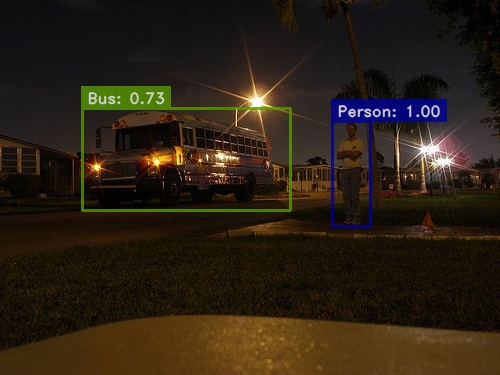
\includegraphics[width=0.2425\linewidth]{samples/good/000231.jpg} \\
      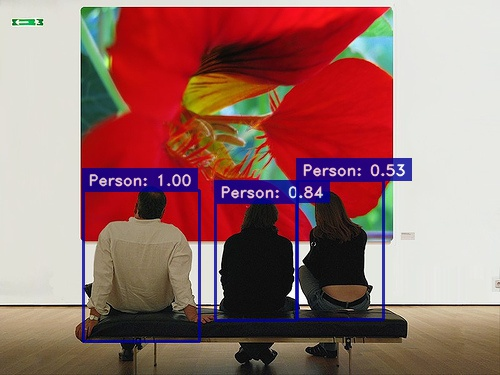
\includegraphics[width=0.2425\linewidth]{samples/good/000279.jpg}
    \end{tabular}\hspace{0.01\linewidth}
    &
    \begin{tabular}{c}
      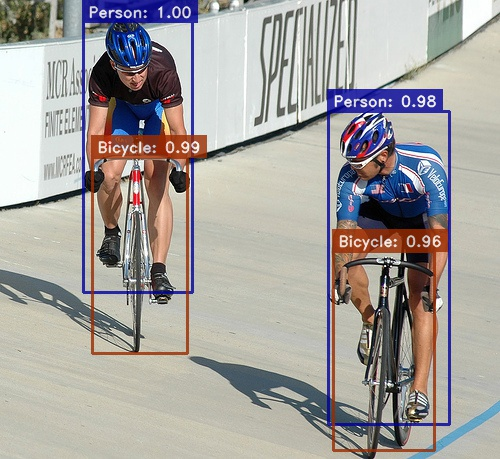
\includegraphics[width=0.2425\linewidth]{samples/good/000283.jpg} \\
      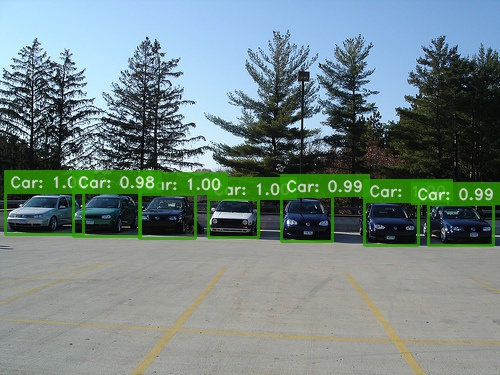
\includegraphics[width=0.2425\linewidth]{samples/good/000313.jpg} \\
      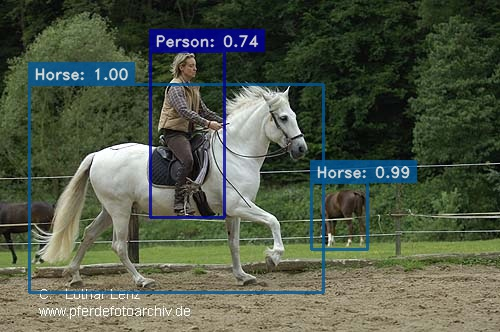
\includegraphics[width=0.2425\linewidth]{samples/good/000319.jpg} \\
      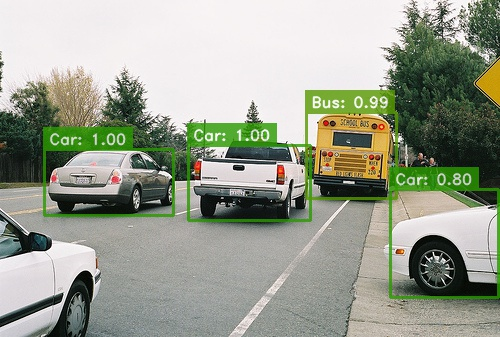
\includegraphics[width=0.2425\linewidth]{samples/good/000341.jpg}
    \end{tabular}\hspace{0.01\linewidth}
    &
    \begin{tabular}{c}
      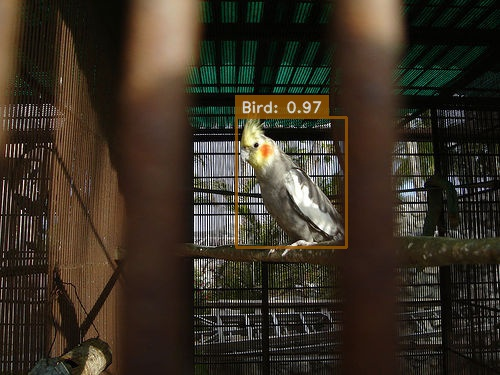
\includegraphics[width=0.2425\linewidth]{samples/good/000466.jpg} \\
      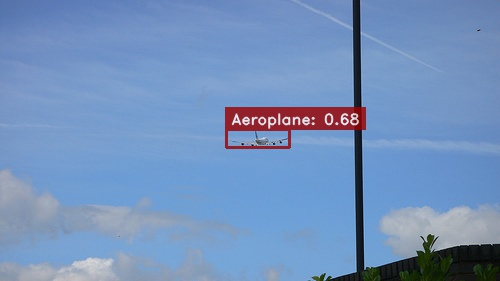
\includegraphics[width=0.2425\linewidth]{samples/good/000817.jpg} \\
      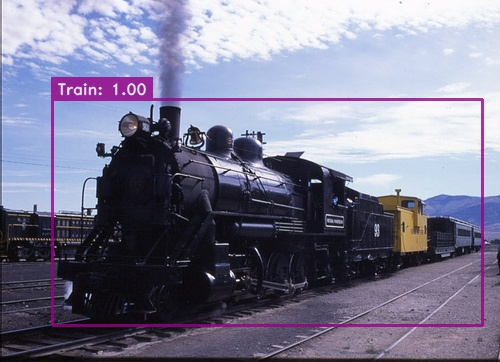
\includegraphics[width=0.2425\linewidth]{samples/good/000824.jpg} \\
      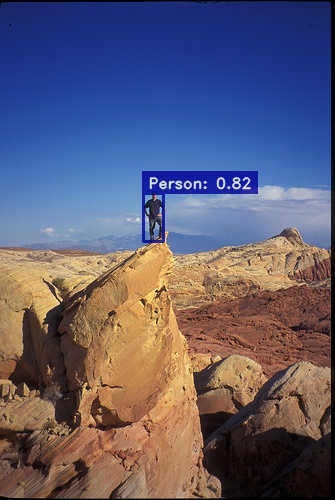
\includegraphics[width=0.2425\linewidth]{samples/good/000869.jpg}
    \end{tabular}
  \end{tabular}
  \captionof{table}{Selected good sample images from Pascal VOC 2007 test set detected by the SSD 300 network.}
\end{center}
\egroup

Objects that were often false classified are animals like cats, cows and dogs. Bottles were also often classified as people. The network has some difficulties to detect groups of objects like people. The predicted bounding boxes often overlap or describe multiple objects.

\bgroup
\setlength\tabcolsep{0pt}
\def\arraystretch{1}
\begin{center}
  \begin{tabular}[t]{cccc}
    \begin{tabular}{c}
      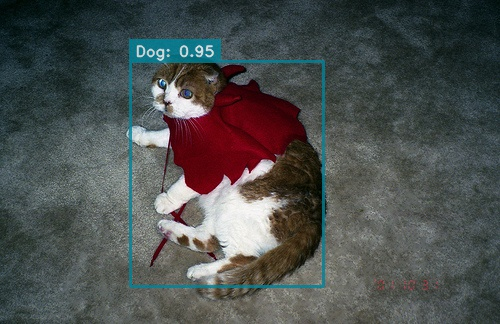
\includegraphics[width=0.2425\linewidth]{samples/bad/000011.jpg} \\
      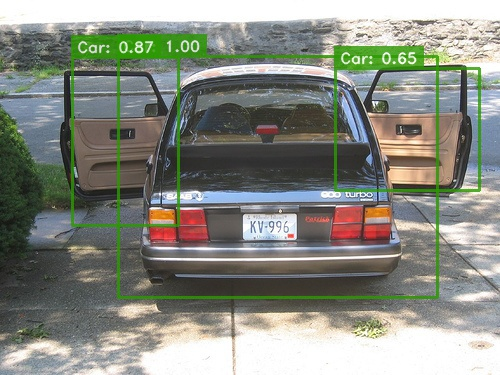
\includegraphics[width=0.2425\linewidth]{samples/bad/000074.jpg} \\
      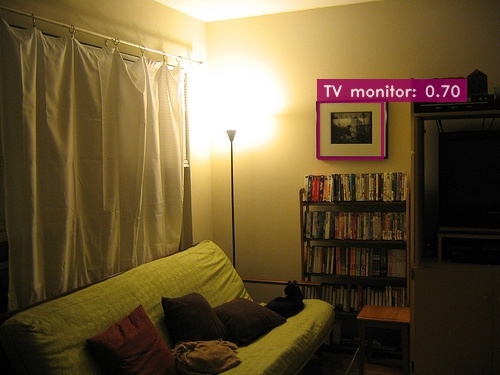
\includegraphics[width=0.2425\linewidth]{samples/bad/000160.jpg}
    \end{tabular}\hspace{0.01\linewidth}
    &
    \begin{tabular}{c}
      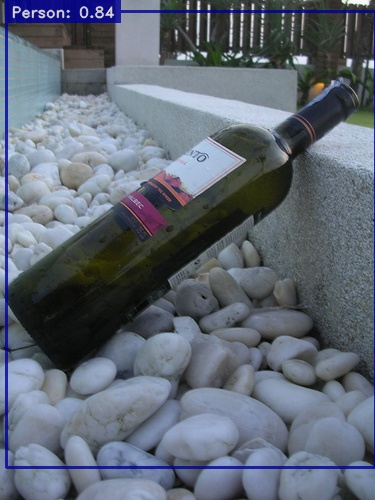
\includegraphics[width=0.2425\linewidth]{samples/bad/000335.jpg} \\
      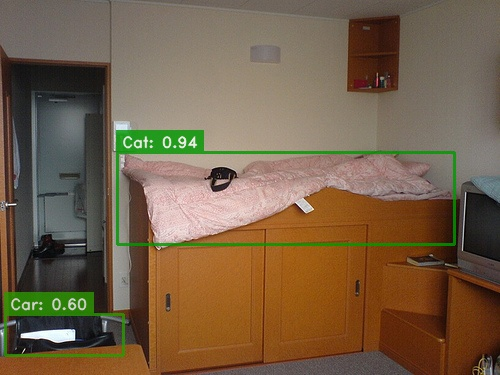
\includegraphics[width=0.2425\linewidth]{samples/bad/001813.jpg}
    \end{tabular}\hspace{0.01\linewidth}
    &
    \begin{tabular}{c}
      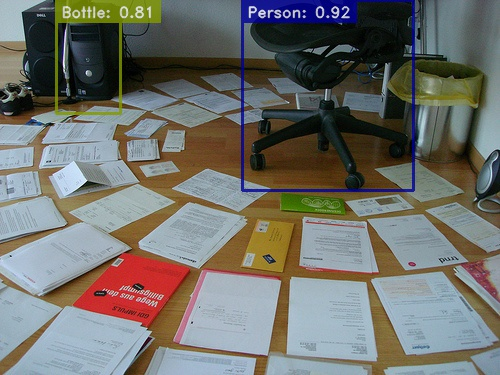
\includegraphics[width=0.2425\linewidth]{samples/bad/001814.jpg} \\
      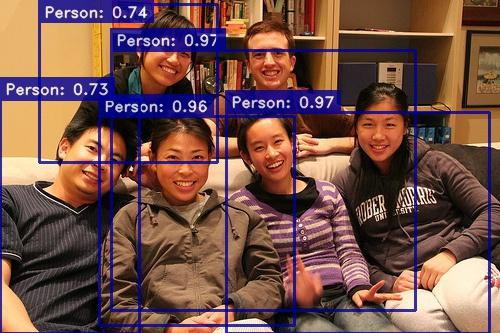
\includegraphics[width=0.2425\linewidth]{samples/bad/000959.jpg} \\
      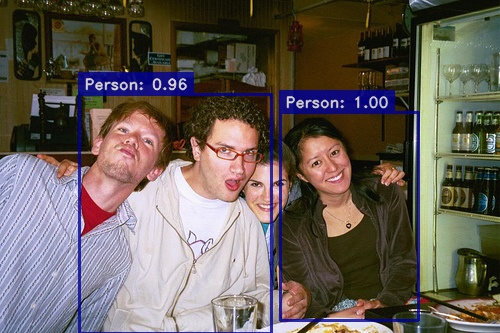
\includegraphics[width=0.2425\linewidth]{samples/bad/002235.jpg}
    \end{tabular}\hspace{0.01\linewidth}
    &
    \begin{tabular}{c}
      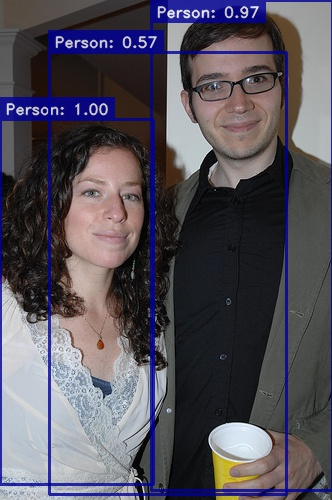
\includegraphics[width=0.2425\linewidth]{samples/bad/000388.jpg} \\
      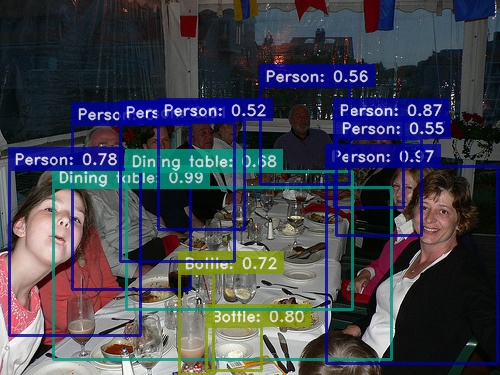
\includegraphics[width=0.2425\linewidth]{samples/bad/000744.jpg}
    \end{tabular}
  \end{tabular}
  \captionof{table}{Selected bad sample images from Pascal VOC 2007 test set detected by the SSD 300 network.}
\end{center}
\egroup
